\documentclass[conference]{IEEEtran}

\usepackage[utf8]{inputenc}
\usepackage[T1]{fontenc}
\usepackage{lmodern}
\usepackage{microtype}
\usepackage{amsmath,amssymb,amsfonts}
\usepackage{graphicx}
\usepackage{booktabs}
\usepackage{multirow}
\usepackage{xcolor}
\usepackage{url}
\usepackage{placeins}
\usepackage[hidelinks]{hyperref}
\usepackage[numbers,sort&compress]{natbib}
\usepackage{stfloats}
\usepackage{caption}
\captionsetup{font=footnotesize}
\captionsetup{skip=2pt}
\usepackage{fancyhdr}
\usepackage{lastpage}

\pagestyle{fancy}
\fancyhf{}
\fancyhead[R]{\thepage}
\fancyhead[L]{CSE756: Probabilistic Graphical Models}
\renewcommand{\headrulewidth}{0.4pt}
\AtBeginEnvironment{equation}{\scriptsize}
\setlength{\abovedisplayskip}{10pt}
\setlength{\belowdisplayskip}{10pt}
\setlength{\abovedisplayshortskip}{4pt}
\setlength{\belowdisplayshortskip}{4pt}
\setlength{\textfloatsep}{8pt}
\setlength{\floatsep}{6pt}
\setlength{\intextsep}{6pt}

 
\title{DualPathCRFNet: End-to-End Learnable CRF with\\
Edge-Aware Fusion for Semantic Segmentation}

\author{
  \IEEEauthorblockN{Md Jawadul Karim}
  \IEEEauthorblockA{MSc. in Computer Science and Engineering\\
    BRAC University, Merul Badda, Dhaka, Bangladesh\\
    \texttt{md.jawadul.karim@g.bracu.ac.bd}}
  \and
  \IEEEauthorblockN{Ipshita Bonhi Upoma}
  \IEEEauthorblockA{Lecturer\\
    BRAC University, Merul Badda, Dhaka, Bangladesh\\
    \texttt{ipshita.upoma@bracu.ac.bd}}
}

\begin{document}
\maketitle

 
\begin{abstract}
Semantic segmentation of complex urban scenes calls for models that are both accurate at the region level
and precise at object boundaries, a conflicting two-points-of-view combined task for standard single-encoder architectures. To this end, we propose a unified end-to-end trainable framework, named
\textbf{DualPathCRFNet}, which overcomes three major limitations of the state-of-the-art approaches: boundary
insensitiveness, spatially inconsistent pixel-wise predictions, and suboptimal multi-stream feature fusion.
Our architecture utilizes a multiple-path encoder consisting of a fine-tuned ResNet-50 backbone for RGB
signal processing, coupled with a dedicated frequency-aware edge branch that explicitly processes Sobel
gradient responses alongside it to support distinct representation learning between semantic information
and boundary structure. Specifically, we propose a scale adaptive fusion strategy which introduces
lightweight concatenation at fine spatial scales and bidirectional cross-attention at coarse scales,
dynamically exchanging complementary information between the two paths where most informative. The
fused features are decoded first with an FPN-style top-down pathway, then are refined by CRF-as-RNN
cascaded at three increasingly fine resolutions to enforce spatial label consistency globally from region
coherence to sharp boundary localization. We train the model on a larger Cityscapes dataset of 15,088
image-mask pairs with a composite loss consisting of cross-entropy, auxiliary supervision, and an explicit
boundary term. On Cityscapes val set, DualPathCRFNet performs with \textbf{70.52\% mIoU}, \textbf{81.62\% mDice},
besides \textbf{94.9\% pixel accuracy}, which contains 34.32M params. The proposed architecture's robustness
beyond the training benchmark is shown by performing an external evaluation on real-time video
sequences from the KITTI dataset, proving the generalizability of the learned representations on unseen
driving scenarios.
\end{abstract}

\begin{IEEEkeywords}
Urban scene understanding, dual-path encoder, frequency-aware edge detection, cross-attention fusion, CRF-as-RNN, Cityscapes, KITTI, autonomous driving, Grad-CAM.
\end{IEEEkeywords}

 
\section{Introduction}\label{sec:intro}

Scene understanding in complex urban environments is one of the most basic and yet difficult problems
in computer vision~\cite{aarthi2017scene}. Semantic segmentation, the problem of labeling a class for each pixel in an image,
is the cornerstone of perception systems used in areas like autonomous driving, smart city infrastructure,
and robot navigation~\cite{hurtado2022semantic}. Errors in these contexts have immediate safety implications; a misclassified
pedestrian, an unnoticed road edge, or a misidentified obstacle can rupture the reliability of the entire
downstream decision pipeline. Thus, the field calls for models that are both accurate and spatially precise,
and that can preserve finer structure detail across the full resolution of the input image. Deep convolutional
neural networks have reached state-of-the-art over the past decade. End-to-end pixel-wise prediction was
established with fully convolutional architectures, while dilated convolutions allowed for large receptive
fields without a loss of spatial resolution. The designs with encoder-decoder architectures having skip
connections recovered partially finer spatial details that have been eroded during encoding. In more recent
years, global context modelling via attention-based architectures has produced competitive segmentation
accuracy across a range of standard benchmarks. While this has made for steady improvements thus far,
several basic constraints remain that no single line of work has adequately addressed, especially in high-resolution, structure-rich scenes like urban driving.

The first of these has to do with boundary sensitivity. Both standard convolution and attention-based
encoders consider the input image as a homogenous signal, where the learnt filters are primarily optimized
to detect textures and the semantic appearance~\cite{scabini2025survey}. On the other hand, object boundaries are inherently
high-frequency events. They appear as high-frequency, abrupt color changes, which are structurally
different from the low-frequency semantic information that dominates most of the image. When a single
encoder is required to capture both regimes, low-frequency semantics often dominate and result in poor
boundary precision. This trade-off is observed in the wild: models get strong region-level accuracy but
produce segmentation maps with jagged, spatially inaccurate boundaries, a critical failure mode wherever
detail structures need to be geometrically localized.

A second limitation has to do with the formality of the output. Traditionally, the dominant decoding
paradigm, pixel-wise classification, processes each spatial location independently by making a conditional
independence assumption among the label probabilities conditioned on local feature vectors. This
fundamentally ignores the rich spatial dependencies across neighboring pixels. In natural scenes, adjacent
pixels nearly always share the same semantic label, and there are structured patterns of label transitions
constrained by object geometry. Decomposing these dependencies leads to locally inconsistent
segmentation maps: isolated misclassified pixels surrounded by correct predictions, spurious label noise
in homogeneous regions, and boundaries that do not respect underlying object contours. Conditional
Random Fields (CRF)~\cite{sutton2012crf} provide a principled probabilistic framework to resolve these inconsistencies
by modeling pairwise interactions between pixels. Still, classical implementations treat the CRF as a
standalone post-processing method, as opposed to an end-to-end trainable building block that can adapt to
the learned feature space. A key contribution of the CRF-as-RNN formulation was to recast mean-field
inference as a differentiable recurrent operation, partially addressing this issue, but most implementations
apply it at a single output resolution, missing the opportunity to enforce spatial consistency progressively,
across scales.

The third limitation relates to the multi-path feature fusion. With the community moving towards multi-stream architectures, pairing semantic encoders with edge detectors, depth estimators, or other auxiliary
branches, the question of how to best fuse these streams rises to the forefront. Naive operators like
element-wise addition or concatenation lack sufficient expressive power to arbitrate between structurally
different sources when combining information from them. Thus at coarsely spatial scales each path's
relative contribution should be adjusted dynamically as a function of the content of each stream. This is
not achievable with naive fusion, and the complementary information carried by different paths are even
likely to compete rather than cooperate.

These three limitations are tangled. The insensitivity of a weak boundary encoder further transmits the
sparse feature representations to the pixel-decoder, where uncooperative pixel classification worsens the
local discrepancies, where misled fusion did not remove its chance to be corrected eternally in the pipeline.
Treating even one of them separately results in only marginal gains; a common model resolving all three
together is needed. In this paper, we propose a semantic segmentation architecture addressing all three
limitations in a single unified end-to-end trainable framework, \textbf{DualPathCRFNet}. We design a dual-head
encoder combining a deep convolutional backbone with a specific frequency-aware edge branch,
processing along-side the RGB signal Sobel gradient responses, enabling focused specialization to
semantic content (labeling head) and boundary structure (edge head). In order to fuse these streams
effectively, we propose a scale adaptive fusion strategy that utilizes lightweight concatenation at fine
spatial scales and bidirectional cross-attention at coarse scales to perform dynamic query-based interaction
between paths where necessary. The decoder then applies CRF-as-RNN refinement at three progressively
increasing resolutions: directly instantiating mean-field variational inference over a dense pairwise
Markov Random Field as a differentiable module which cascades from global consistency at low
resolution to sharp boundary localization at full resolution. An explicit boundary loss serves this purpose
on the edge branch, acting as an additional learning signal when compared to the region-level cross-entropy used at the segmentation heads.

 
\section{Literature Review}\label{sec:lit}

Semantic segmentation of urban and complex scenes has seen substantial methodological diversity, with
researchers exploring fully supervised, semi-supervised, weakly supervised, and real-time approaches,
each addressing a distinct bottleneck in the segmentation pipeline.

A foundational line of work focuses on encoder-decoder architectures applied directly to urban
benchmarks. Arulananth et al.~\cite{arulananth2024unet} demonstrated that a carefully regularized U-Net outperforms FCN,
ENet, and DeepLabV3 baselines. However, their model was trained from scratch at low resolution
(128$\times$128), and the authors themselves noted that IoU overfitting emerged after 20--25 epochs, suggesting
the architecture's ceiling is constrained by input scale and training depth. In a structurally related effort,
Guo and Dou~\cite{guo2021segnet} embedded CRF-as-RNN mean-field inference directly as the final layer of SegNet,
replacing the decoupled post-processing paradigm. Their end-to-end framework produced sharper
boundaries on KITTI-Road and a zebra-crossing dataset, confirming that joint optimization of feature
extraction and spatial regularization is preferable to treating CRF as an afterthought. An et al.~\cite{an2023crfnet} extended
this philosophy further by proposing CRFNet, a context refinement module attachable to any existing
encoder-decoder backbone. Using dilated convolutions and context pooling to process label-level spatial
context, then fusing with penultimate backbone features, CRFNet consistently improved mIoU across
Cityscapes, CamVid, and KITTI-360 with minimal parameter overhead, demonstrating that refinement
can be architecturally decoupled from the backbone without sacrificing learning coherence.

Complementing these fully supervised approaches, several works have explored how to reduce annotation
dependency while maintaining segmentation quality. Huang et al.~\cite{huang2021hyperspectral} leveraged hyperspectral imagery to
circumvent the metamerism limitation of RGB cameras, where distinct objects share visually identical
pixel values. By training a ResNet-50 classifier on hyperspectral cubes to generate spectral priors, then
fusing these with coarse polygon labels via class-wise erosion, they produced refined training labels that
improved HRNet mIoU by over 10\% on the Hyperspectral City dataset. Similarly, Maggiolo et al.~\cite{maggiolo2021semisupervised}
addressed scribble-supervised segmentation of very-high-resolution aerial images by proposing a cluster-level fully connected CRF that approximates long-range pixel dependencies using PCA-reduced CNN
activations and k-means clustering. On the ISPRS Vaihingen and Potsdam benchmarks, their Cl-FC-CRF
partially closed the gap between scribble-trained and densely supervised models. Gao et al.~\cite{gao2022offroad} pushed
further into the weakly supervised regime for off-road scenes, combining contrastive learning, adaptive
Gaussian-mixture clustering, and active learning to achieve performance comparable to fully supervised
baselines with as few as 40 annotated frames, applying DenseCRF optionally to refine boundaries.

The challenge of training label bias was directly addressed by He et al.~\cite{he2021dars}, who demonstrated that
standard self-training pseudo-labels are heavily skewed toward majority classes due to long-tailed
distributions. Their DARS method, combining class-specific confidence thresholds with random
sampling, aligned pseudo-label distributions with true label distributions, yielding an 8.89\% mIoU gain
on Cityscapes with only 1/8 labeled data. This complements the data-side augmentation strategy explored
by Sahin et al.~\cite{sahin2023multispectral}, who showed that targeted spectral channel selection (Green, Filtered-NIR, NDVI)
combined with fully connected CRF post-processing improved boundary-level precision in crop/weed
segmentation, achieving a mean IoU of 0.883.

For real-time deployment, Yu et al.~\cite{yu2018bisenet} proposed BiSeNet, which decouples spatial detail preservation
and receptive field coverage into a Spatial Path and a Context Path, respectively, achieving 68.4\% mIoU
at 105 FPS on Cityscapes, establishing that architectural path specialization, rather than input downsampling or channel pruning, is the more principled route to real-time segmentation. Zhang et al.~\cite{zhang2023sar}
applied a related dual-path philosophy to SAR change detection, using a dual-encoder network with
dynamic convolution kernels and a CRF model whose pairwise potentials are guided by local boundary
entropy, outperforming transformer and CNN baselines across four SAR datasets.

 
\section{Methodology}\label{sec:method}

\subsection{Dataset and Preprocessing}\label{subsec:data}

This work is largely based on a single dataset: the Cityscapes dataset~\cite{cordts2016cityscapes}, a large-scale, fine-grained
benchmark for urban scene understanding. Cityscapes contains high-resolution images (2048$\times$1024)
acquired from a car-mounted camera on the road in 50 different cities in Europe with dense pixel-level
annotations, which allows for 19 semantic classes of objects to be annotated (road, sidewalk, building,
vehicle types, pedestrian, vegetation etc.). The standard split includes 2,975 meticulously annotated training
images and 500 validation images, along with their associated label mask for semi-supervised
segmentation. Cityscapes is a standard benchmark, but with only 2,975 training images, the dataset is
small within the current norms of deep learning, and the dataset has an apparent visual bias since a large
portion of the images were taken in overcast or low-light situations, leading to lower colors, lower contrast,
and less visible boundaries. However, training a model with a frequency-aware edge branch on such data
risks underfitting the edge pathway since dark low-contrast images respond weakly to Sobel gradients,
providing minimal structural information. We tackle both the small number of instances and the visual
bias via the application of an offline augmentation technique on the training set through a multi-stage
pipeline. The validation set stays the same all the time.

All training image and label mask pairs are horizontally flipped, generating a mirrored pair for each. This
more than doubles the training set from 2,975 image-mask pairs to 5,950 image-mask pairs. The class
labels that represent vehicles and road surfaces, which are the primary targets of this method, are
semantically symmetric with respect to left-right reflection, making horizontal flipping safe for the traffic
conditions present in the Cityscapes label space, truth labels, 3D rendered images, and other classes present
in the label space won't change.

The second step includes the application of a photometric enhancement pipeline that produces brightened
versions of the original (non-flipped) images. The enhancement includes gray-world white balance
correction in color space to remove color casts; CLAHE (Contrast-Limited Adaptive Histogram
Equalization) to increase local contrast with a clip limit of 2.5 and 8$\times$8 tile grid. The resulting images are
visually overall brighter, more saturated, and with a greater local contrast than the originals, exactly the
conditions when Sobel gradients produce more pronounced and informative edge responses. The original
label mask for every brightened image is kept unchanged, because photometric transforms such as shift,
reflection and scaling do not affect the geometry of objects. We use a perceptual hash filter to stop the
augmentation from introducing near-duplicate images, which would inflate the training count without
genuinely increasing diversity. For every brightened image, we calculate its perceptual hash (pHash) and
compare the hash of the original against it. We only keep pairs whose Hamming distance is bigger than 9.
This guarantees every augmented sample kept and added to the distribution contains noticeably different
and visual content during training.

The third stage involves the creation of crops of every accumulated image (the originals, mirrored, and
brightened copies that are retained). For each image, a 2048$\times$1024 center crop is taken horizontally (304
pixels removed from either side) and vertically anchored at the top (720 upper image rows retained) to
form a 1440$\times$720 output. This crop discards the vehicle hood seen at the bottom of most Cityscapes frames,
as well as regions in the image that typically contain fewer informative objects, while keeping the central
driving scene where most annotated objects are located. The cropped images are simply used as extra
training examples with the full size originals, allowing the model to be trained with a different spatial scale
/ aspect ratio. As such, following all augmentation steps, the final train set is composed by \textbf{15,088 image-masks pairs}. The size of the validation set stays at 500 unaugmented pairs.
Figure~\ref{fig:classdist} shows the class-wise pixel distribution of the Cityscapes augmented dataset (train + val).

\begin{figure*}[!t]
  \centering
  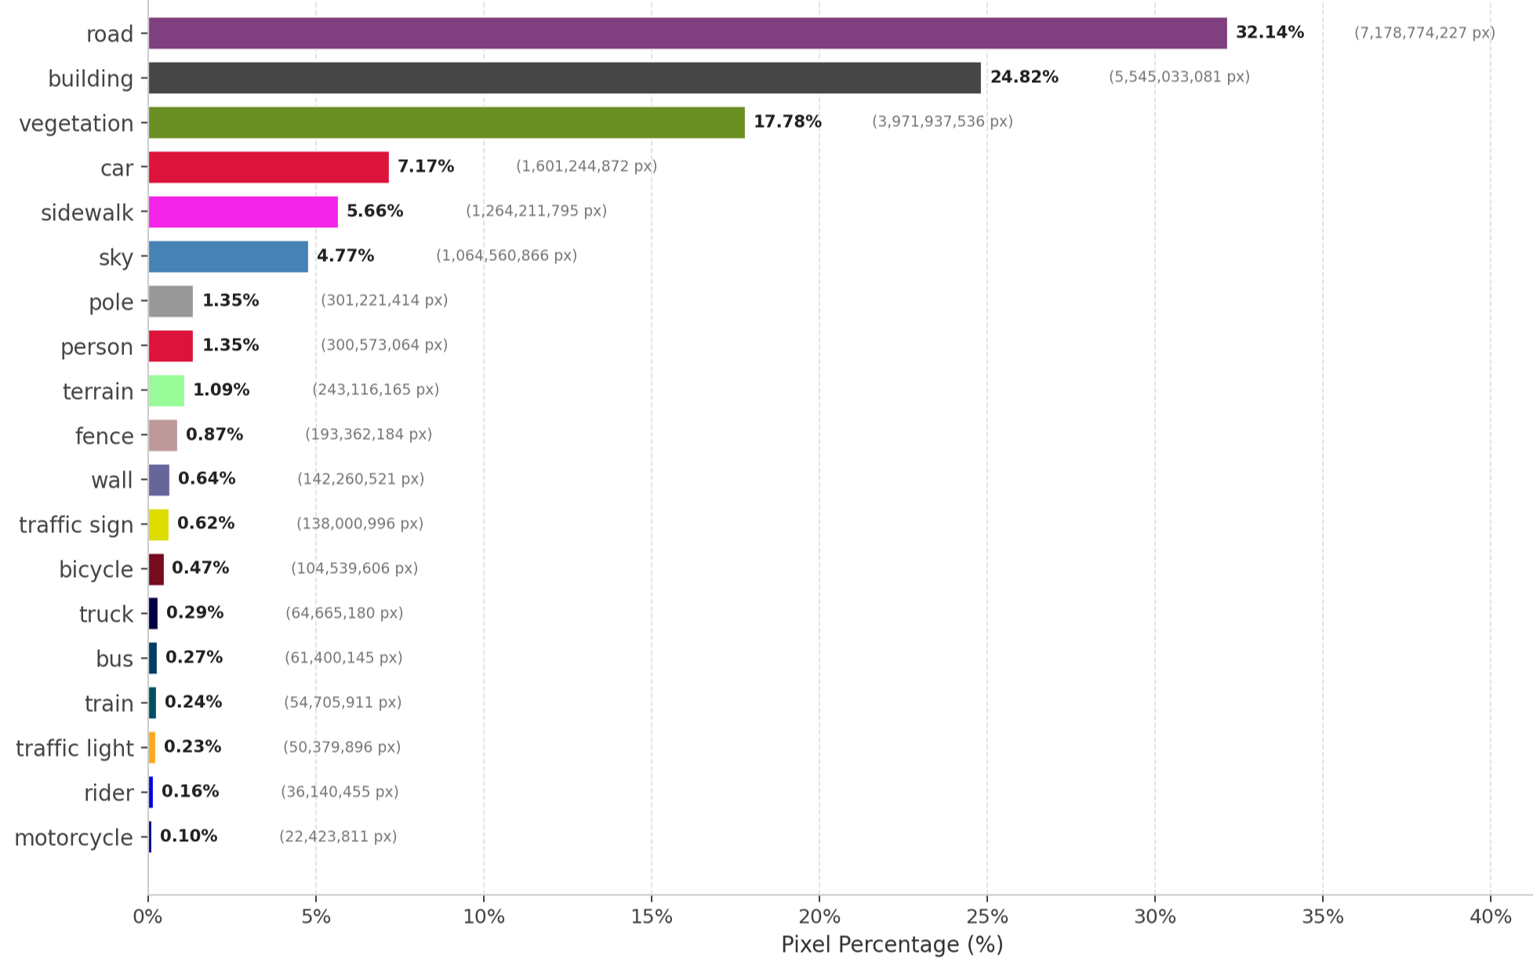
\includegraphics[width=0.8\textwidth]{Picture1.png}
  \caption{Class-wise pixel distribution of the Cityscapes augmented dataset (train + val).}
  \label{fig:classdist}
\end{figure*}

\begin{figure*}[!b]
  \centering
  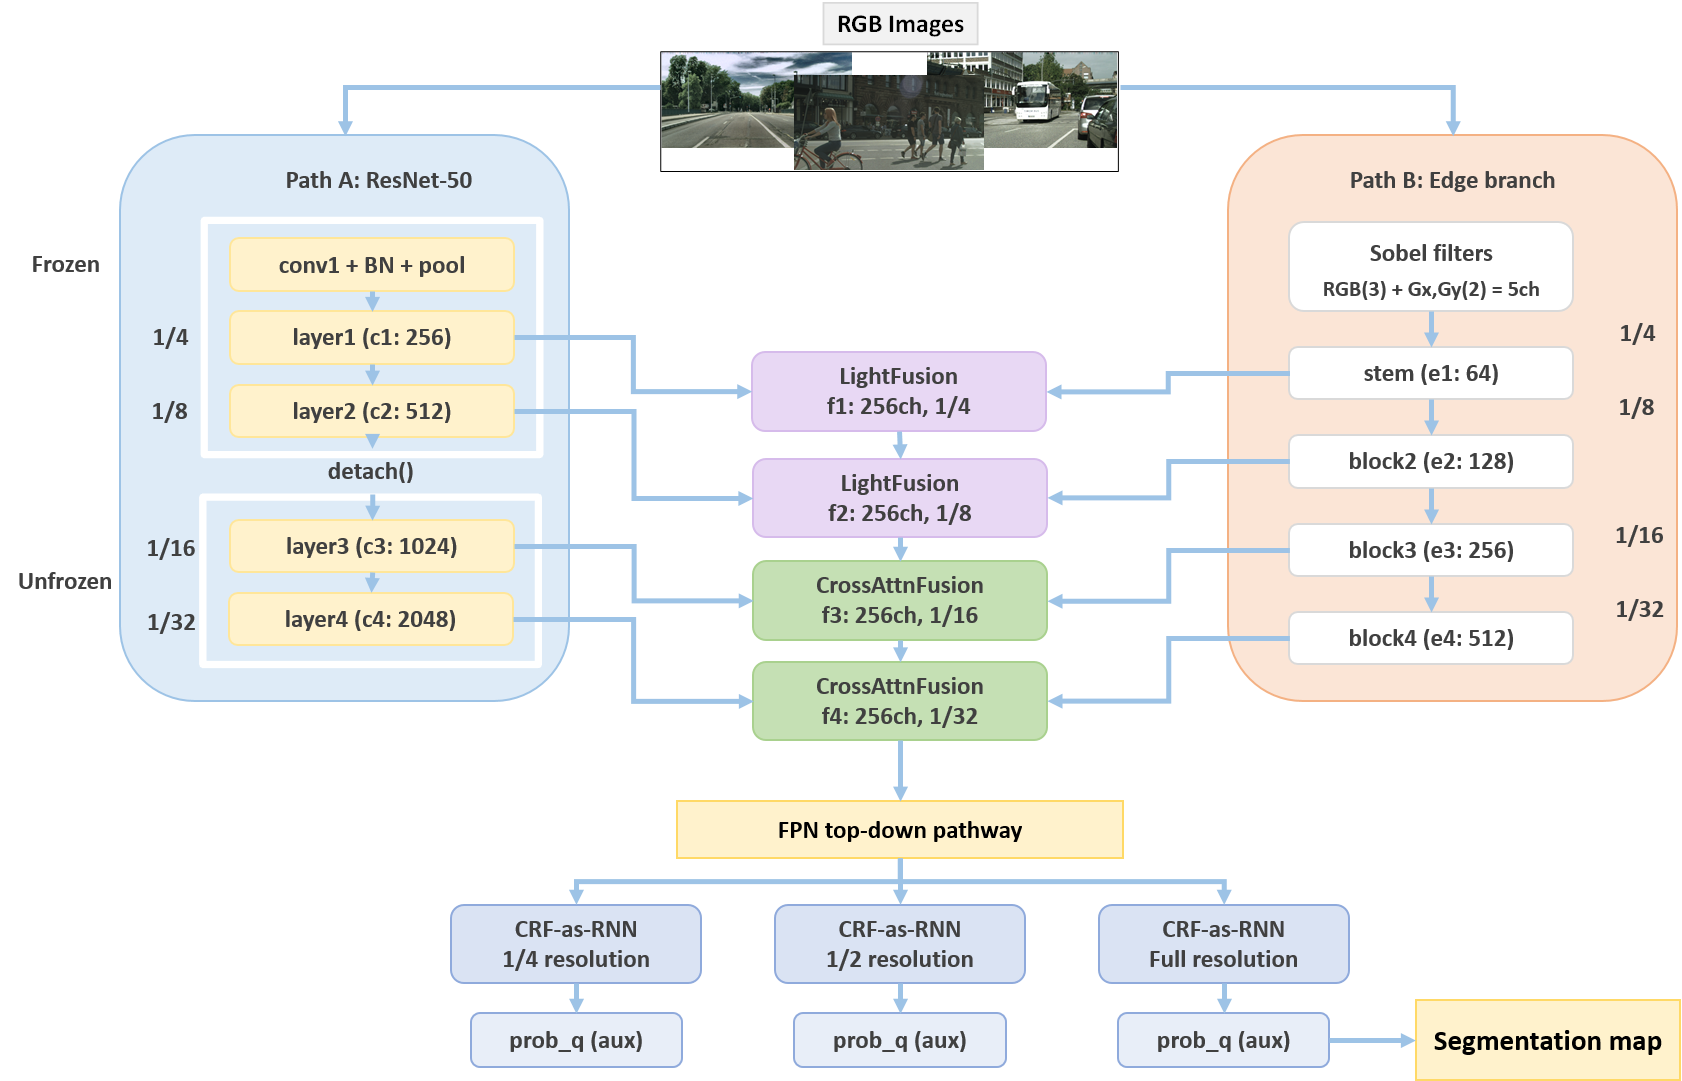
\includegraphics[width=.8\textwidth]{Picture2.png}
  \caption{DualPathCRFNet overall architecture diagram showing dual-path encoder, scale-adaptive fusion, and multi-scale CRF decoder.}
  \label{fig:architecture}
\end{figure*}

\subsection{Model Architecture}\label{subsec:arch}

This section describes the DualPathCRFNet architecture in detail.
The model consists of four major components: (1) a dual-path encoder comprising
a ResNet-50~\cite{he2016resnet} backbone and a frequency-aware edge branch,
(2) a scale-adaptive fusion strategy, (3) a feature pyramid decoder with
multi-scale CRF-as-RNN refinement, and (4) a composite loss function.
Based on Figure~\ref{fig:architecture}, given an input RGB image $\mathbf{x} \in \mathbb{R}^{3\times H\times W}$,
DualPathCRFNet produces a pixel-wise class probability map
$\hat{\mathbf{y}} \in \mathbb{R}^{C\times H\times W}$, where $C = 19$ is the
number of semantic classes. The image is simultaneously passed through Path~A (the
convolutional backbone) and Path~B (the edge branch). Each path produces feature maps at four spatial
scales: 1/4, 1/8, 1/16, and 1/32 of the input resolution. At each scale, the two feature streams are merged
by a fusion module. The four fused feature maps then feed into a Feature Pyramid Network
(FPN)~\cite{kirillov2019fpn} decoder, which produces predictions at three increasing resolutions. Each prediction is refined by a CRF-as-RNN module that performs differentiable mean-field inference. The final segmentation is taken from
the full-resolution CRF output.

\begin{figure}[!b]
  \centering
  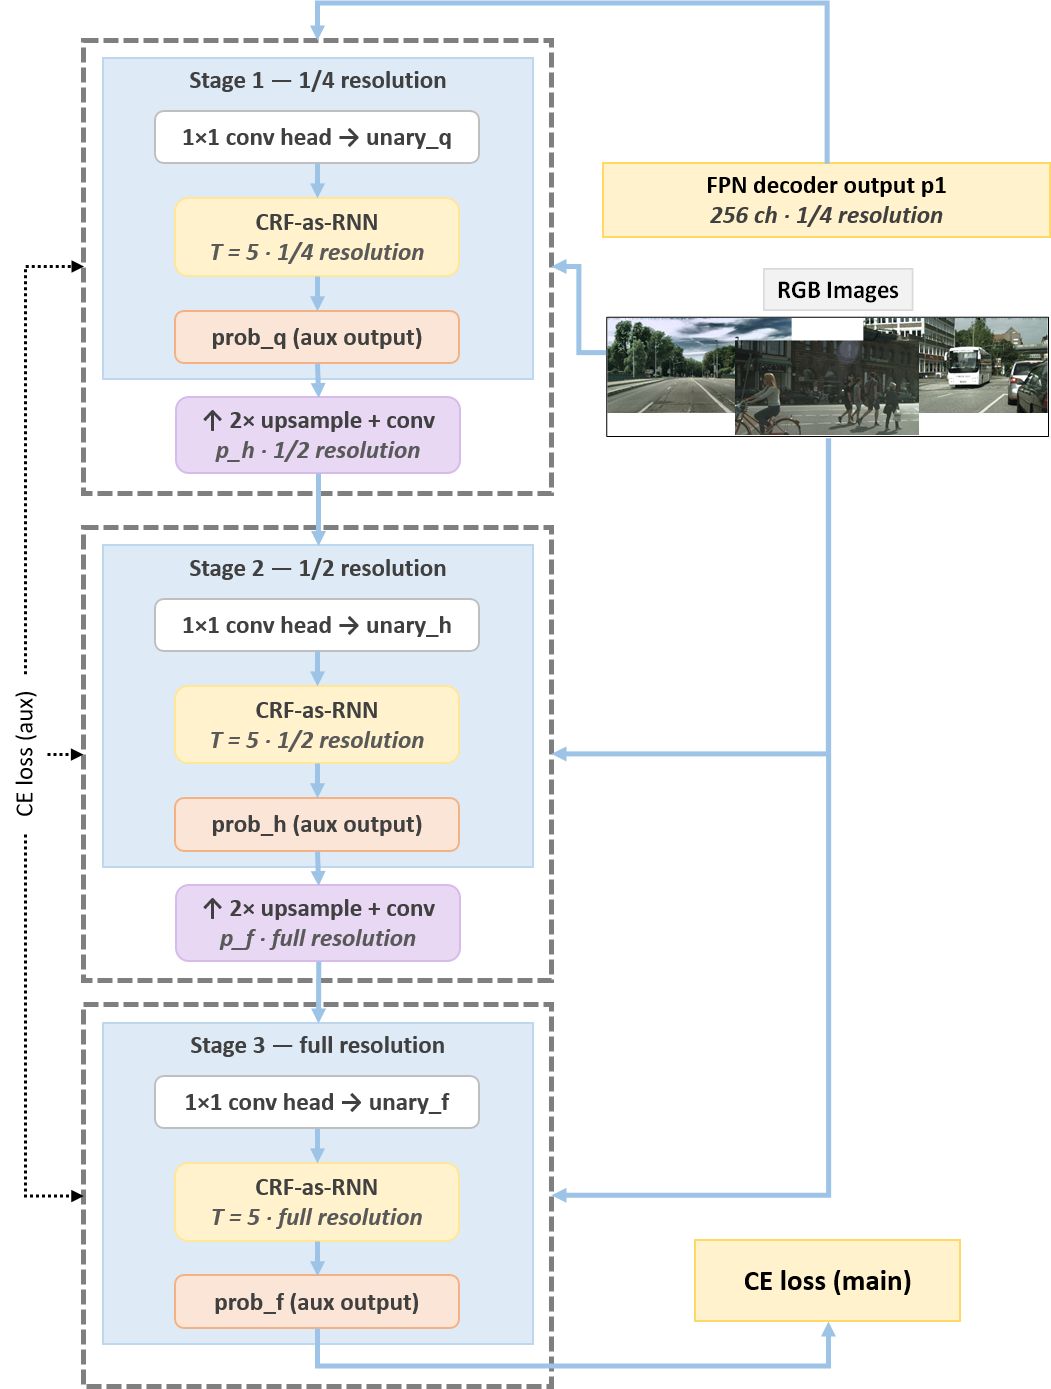
\includegraphics[width=\columnwidth]{Picture3.png}
  \caption{Multi-scale CRF-as-RNN decoder pipeline with three progressive
           refinement stages at 1/4, 1/2, and full resolution.}
  \label{fig:crfdecoder}
\end{figure}

\subsubsection{Path A --- ResNet-50 Semantic Backbone}
Path~A uses a ResNet-50 pretrained on ImageNet as a hierarchical feature extractor. We denote the four
residual stage outputs as $c_1, c_2, c_3, c_4$ with channel dimensions 256, 512, 1024, and 2048 at spatial scales
1/4, 1/8, 1/16, 1/32, respectively. Each residual block computes:
\begin{equation}
  h_l = \sigma\!\left(F(h_{l-1};\,W_l) + S(h_{l-1})\right),
  \label{eq:resblock}
\end{equation}
where $F(\cdot;\,W_l)$ is the learned residual mapping (a stack of convolutions with weights $W_l$), $S(\cdot)$ is the
shortcut connection (identity or $1\!\times\!1$ projection), and $\sigma$ is ReLU. The residual design allows
gradient flow through skip paths, which is critical for training deep networks on dense prediction tasks
where gradients must propagate back through many layers to update low-level feature representations.

We partition the backbone into frozen and unfrozen zones. The stem, layer1, and layer2 are frozen: their
parameters are fixed at ImageNet-pretrained values, batch normalization statistics are locked in eval mode,
and gradients are detached after layer2:
\begin{equation}
  c_3 = \mathrm{layer3}\!\left(\mathrm{detach}(c_2)\right).
  \label{eq:detach}
\end{equation}
This prevents any gradient from flowing into the frozen layers. Layer3 and layer4 remain trainable but
receive a reduced learning rate (0.3$\times$ the base rate). This design is motivated by the observation that early
convolutional layers learn generic low-level features that transfer well across tasks without modification,
while deeper layers encode task-specific semantics that benefit from fine-tuning on the target domain.

\subsubsection{Path B --- Frequency-Aware Edge Branch}
Object boundaries are high-frequency signals that standard convolutional backbones tend to suppress
through repeated pooling and large receptive fields. Path~B is designed to explicitly preserve this frequency
information. Given input image $\mathbf{x}$, we first compute horizontal and vertical Sobel gradients:
\begin{equation}
  G_x = K_x * I_{\mathrm{gray}}, \quad G_y = K_y * I_{\mathrm{gray}},
  \label{eq:sobel}
\end{equation}
where $I_{\mathrm{gray}}$ is the luminance conversion, $K_x$ and $K_y$ are the
standard $3\!\times\!3$ Sobel kernels, and $*$ denotes 2D convolution. The gradient maps are concatenated with the original RGB channels to form a
5-channel input:
\begin{equation}
  \mathbf{z} = [\mathbf{x};\,G_x;\,G_y] \in \mathbb{R}^{5\times H\times W}.
  \label{eq:5ch}
\end{equation}
This 5-channel tensor is then processed by a lightweight convolutional network consisting of a stem (two
stride-2 convolutions to reach 1/4 scale) followed by three downsampling blocks, producing edge features
$e_1, e_2, e_3, e_4$ at the same four spatial scales as Path~A, with channel dimensions 64, 128, 256, 512. Each
block applies:
\begin{equation}
  e_k = \sigma\!\left(\mathrm{BN}\!\left(\mathrm{Conv}_{3\times3}(e_{k-1},
        s\!=\!2)\right)\right)
        \!\to\!
        \sigma\!\left(\mathrm{BN}\!\left(\mathrm{Conv}_{3\times3}(\cdot)\right)\right),
  \label{eq:edgeblock}
\end{equation}
where $s=2$ is the stride for spatial downsampling, BN is batch normalization, and $\sigma$ is ReLU. The explicit
inclusion of Sobel features means the edge branch receives a direct high-frequency prior at its input,
allowing it to specialize in boundary structure without competing against the dominant low-frequency
semantics that the backbone encodes. An auxiliary edge head ($1\!\times\!1$ convolution) is attached to $e_1$ to
produce a single-channel boundary prediction supervised with a dedicated loss term.

\subsubsection{Scale-Adaptive Fusion}
The fusion strategy varies by spatial scale.
At fine scales (1/4 and 1/8), where feature maps are spatially large, we use
\emph{LightFusion}, a concatenation followed by a $1\!\times\!1$ convolution:
\begin{equation}
  f_k = \sigma\!\left(\mathrm{BN}\!\left(W_{1\times1}\cdot[c_k;\,e_k]\right)\right),
  \label{eq:lightfusion}
\end{equation}
where $W_{1\times1}$ is a $1\times1$ convolution projecting from $(\mathrm{dim}_A + \mathrm{dim}_B)$ channels to the output dimension (256). This is
computationally efficient at high spatial resolutions where the token count would make attention
prohibitive. At coarse scales (1/16 and 1/32), where spatial dimensions are small enough to admit quadratic
attention, we use \emph{CrossAttnFusion}~\cite{li2024crossfuse}. Both feature streams are first projected to a common dimension $d$,
then flattened to sequences and passed through bidirectional multi-head cross-attention:
{\scriptsize
\begin{align}
  \hat{a} &= \mathrm{MHA}(Q\!=\!a,\,K\!=\!b,\,V\!=\!b), \label{eq:mha1}\\
  \hat{b} &= \mathrm{MHA}(Q\!=\!b,\,K\!=\!a,\,V\!=\!a), \label{eq:mha2}
\end{align}
}
where $a$ and $b$ are the projected and layer-normalized feature sequences from
Path~A and Path~B, respectively, and MHA denotes multi-head attention with 4 heads. The multi-head attention itself
computes:
\begin{equation}
  \mathrm{Attention}(Q,K,V) = \mathrm{softmax}\!\left(\frac{QK^\top}{\sqrt{d_k}}\right) V,
  \label{eq:attention}
\end{equation}
where $d_k = d/\text{num\_heads}$ is the per-head dimension. The attended representations are concatenated and passed
through a feed-forward network:
\begin{equation}
  f_k = \mathrm{LN}\!\left(\mathrm{FFN}\!\left([(a+\hat{a});\,(b+\hat{b})]\right) + a\right),
  \label{eq:crossattn_out}
\end{equation}
where FFN is a two-layer network with GELU activation, and LN is layer normalization. The residual connection
from $a$ ensures that the original semantic features are preserved even when the cross-attention mechanism
identifies limited complementary information. This bidirectional design allows each path to selectively
query the other: the backbone can attend to edge features to sharpen its representations at boundaries, and
the edge branch can attend to semantic features to disambiguate intra-class edges from inter-class
boundaries.

\subsubsection{Multi-Scale CRF-as-RNN Decoder}
This is the core probabilistic graphical model component of DualPathCRFNet. A dense CRF defines a
probability distribution over label assignments by combining unary potentials (per-pixel evidence from
the network) with pairwise potentials (compatibility constraints between neighboring pixels). The CRF
energy for a label assignment $\mathbf{y}$ over $N$ pixels is:
\begin{equation}
  E(\mathbf{y}) = \sum_i \psi_u(y_i) + \sum_{i \neq j} \psi_p(y_i, y_j),
  \label{eq:crfenergy}
\end{equation}
where $\psi_u(y_i) = -U_i(y_i)$ is the unary potential derived from the decoder
logits and $\psi_p$ is the pairwise potential that penalizes inconsistent label assignments between spatially
close pixels. Exact inference in a dense CRF is intractable because the pairwise term connects all pixel
pairs. Mean-field variational inference approximates the true posterior
$P(\mathbf{y}|\mathbf{x})$ with a fully factored distribution
$Q(\mathbf{y}) = \prod_i Q_i(y_i)$, minimizing the KL divergence $\mathrm{KL}(Q \| P)$. The mean-field update for pixel $i$ at iteration $t+1$ is:
\begin{equation}
  Q_i^{t+1}(l) = \frac{1}{Z_i}\exp\!\left(-\psi_u(l)
    - \sum_{j}\sum_{l'}\mu(l,l')\sum_m w_m k_m(f_i,f_j)Q_j^t(l')\right),
  \label{eq:mfupdate}
\end{equation}
where $\mu(l, l')$ is the label compatibility function, $k_m$ are the filter kernels, $w_m$ are their learnable weights,
$f_i$ and $f_j$ are feature vectors at pixels $i$ and $j$, and $Z_i$ is a normalization constant. In our CRF-as-RNN
implementation, we approximate the dense pairwise filtering with two convolutional operations rather
than the permutohedral lattice~\cite{kiefel2014permutohedral} used in classical dense CRF implementations. This is the key
architectural difference from the standard CRF. Instead of bilateral filtering over a high-dimensional
feature space, we use two message-passing kernels. The \emph{smoothness message} is a depthwise convolution with a learned
Gaussian kernel applied to $Q^t$:
\begin{equation}
  m_{\mathrm{smooth}} = \mathrm{Conv}_{k\times k,\,\mathrm{groups}=C}(Q^t).
  \label{eq:msmooth}
\end{equation}
This operation applies a separate $K\times K$ ($K=5$) spatial filter to each class channel independently,
approximating the Gaussian spatial kernel that encourages nearby pixels to take the same label regardless
of appearance. The \emph{appearance message} is a standard convolution applied to the
concatenation of $Q^t$ and the RGB image:
\begin{equation}
  m_{\mathrm{appear}} = \mathrm{Conv}_{k\times k}([Q^t;\,I]).
  \label{eq:mappear}
\end{equation}
This kernel is conditioned on both the current marginals and the image appearance, approximating the
bilateral kernel that encourages pixels with similar color and spatial proximity to share labels. The image
conditioning means that edges in the input, color discontinuities, naturally suppress the smoothing effect,
preserving boundaries. The total pairwise message is a weighted combination followed by the
compatibility transform:
\begin{equation}
  \mathrm{pairwise} = W_{\mathrm{compat}}\cdot
                      (w_s\cdot m_{\mathrm{smooth}} + w_a\cdot m_{\mathrm{appear}}),
  \label{eq:pairwise}
\end{equation}
where $w_s$ and $w_a$ are learnable scalar weights and $W_{\mathrm{compat}}$
is a $C\!\times\!C$ $1\!\times\!1$ convolution (the compatibility matrix).
This completes one mean-field iteration. The module runs $T = 5$ iterations before producing the final
output probabilities. Rather than applying the CRF at a single resolution, we cascade it across three scales
shown in Figure~\ref{fig:crfdecoder}. From $p_1$ at 1/4 resolution, a classification head produces unary logits that are refined
by the first CRF to yield $\mathrm{prob}_q$. The features are then upsampled $2\times$ and passed through a lightweight
convolution to produce the 1/2-scale unary, refined by a second CRF to yield $\mathrm{prob}_h$. A final $2\times$ upsample
and convolution produce the full-resolution unary, refined by the third CRF to yield $\mathrm{prob}_f$, the final
prediction. Each CRF operates independently with its own learned parameters, allowing each to specialize
to the error patterns at its resolution. The coarse-scale CRF resolves large-region misclassifications while
the full-resolution CRF focuses on boundary alignment and small-object recovery. This multi-scale
cascade is motivated by the observation that segmentation errors are scale-dependent, coarse errors require
global context to correct, while fine errors require high-resolution spatial detail.

\subsection{Training Configuration}\label{subsec:training}

Table~\ref{tab:hparams} lists the hyperparameters used for training.
The composite loss combines the main cross-entropy loss on $\mathrm{prob}_f$,
auxiliary cross-entropy losses ($\lambda_{\mathrm{aux}} = 0.4$) on
$\mathrm{prob}_q$ and $\mathrm{prob}_h$, and an explicit boundary term
($\lambda_{\mathrm{edge}} = 0.2$) on the auxiliary edge head output.

\begin{table}[!t]
  \centering
  \caption{Training Hyperparameters.}
  \label{tab:hparams}
  \footnotesize
  \begin{tabular}{@{}ll@{}}
    \toprule
    \textbf{Hyperparameter} & \textbf{Value} \\
    \midrule
    Input resolution        & $512 \times 1024$ \\
    Batch size              & 4 \\
    Optimizer               & AdamW \\
    Base learning rate      & $1 \times 10^{-4}$ \\
    Backbone learning rate  & $3 \times 10^{-5}$ (0.3$\times$ base) \\
    Weight decay            & $1 \times 10^{-4}$ \\
    LR schedule             & Cosine annealing w/ linear warmup \\
    Warmup epochs           & 5 \\
    Total epochs            & 60 \\
    Mixed precision         & FP16 \\
    Gradient clipping       & Max norm 1.0 \\
    Auxiliary loss ($\lambda_{\mathrm{aux}}$) & 0.4 \\
    Edge loss ($\lambda_{\mathrm{edge}}$)     & 0.2 \\
    CRF iterations ($T$)    & 5 \\
    CRF kernel size ($K$)   & $5 \times 5$ \\
    Early stopping patience & 5 epochs (on val mIoU) \\
    \bottomrule
  \end{tabular}
\end{table}

\subsection{Evaluation Metrics}\label{subsec:metrics}

We assess DualPathCRFNet based on three complementary numerical metrics, mean Intersection over
Union (mIoU), mean Dice coefficient (mDice) and pixel accuracy, and different kinds training/validation
plots that together tell us the entire story about the performance of the model, the dynamics of the learning
process, and the role of the CRF refinement stage. Mean Intersection over Union (mIoU) is the main metric
and also the standard benchmark measure for semantic segmentation on Cityscapes. For instance, in urban
scenes classes such as truck, train and motorcycle take up far less pixels than road or building; to avoid
this, mIoU weights classes equally making sure that predominant classes do not overshadow performance.
Mean Dice coefficient offers another perspective on overlap quality. Dice has the same per-class
computation structure as IoU, but with a greater weight on true positives and induces greater sensitivity
for classes that are already well-segmented compared to the IoU loss. mIoU punishes both oversegmentation and under-segmentation equally, while mDice is slightly more forgiving of the imprecision
of segment boundaries and thus facilitates distinguishing whether gains in mIoU result from improved
recall or precision. Pixel accuracy is defined as the ratio of correctly predicted pixels to the total number
of pixels. This is more of a sanity check than an actual metric. A model that represents every pixel as a
road (regardless of what the data looks like) could have high pixel accuracy by convention as a metric but
would be useless for practical segmentation. We report it for completeness and as a sanity check that
increases in mIoU are not offset by regressions in overall classification rate. All these metrics and
visualizations together can help analyze final segmentation quality, but also the overall learning stability,
if the marginal value of CRF refinement is worth the computation time, and the distribution of performance
at the class-level.

 
\section{Result \& Analysis}\label{sec:results}

\subsection{Quantitative Results}\label{subsec:quant}

In Table~\ref{tab:results}, we present quantitative results of DualPathCRFNet on the
Cityscapes validation set. CRF-refined the mean IoU improves from 68.60\% to 70.52\% (+1.92 percentage points), indicating the
effectiveness of the multi-scale CRF-as-RNN decoder. This indicates that the learnable mean-field
inference learns some more spatial regularization beyond that learned by the FPN decoder. Meanwhile,
the mDice scores achieve a similar trend, improving from 80.09\% to 81.62\% after CRF, which further
verifies that our model also has better boundary alignment and region consistency. The pixel accuracy
achieves 94.9\%, meaning that most of the pixels are correctly classified at a global level. Regarding
efficiency, the parameter numbers (34.32M) and model size (391 MB) of DualPathCRFNet are also
competitive for a dual-path model with bidirectional cross-attention and three cascaded CRF modules. Its
inference time is 103.2 ms/image (at 512$\times$1024 resolution), which is ok for any non-real-time perception
application (offline-mapping/scene analysis pipeline). Safe to say, these results suggest DualPathCRFNet
strikes a good balance between segmentation accuracy and computational expense on a challenging urban
driving benchmark.

\begin{table}[!b]
  \centering
  \caption{Quantitative Results on Cityscapes Validation Set.}
  \label{tab:results}
  \footnotesize
  \begin{tabular}{@{}lc@{}}
    \toprule
    \textbf{Metric} & \textbf{Value} \\
    \midrule
    mIoU (After CRF)     & 70.52\% \\
    mIoU (Before CRF)    & 68.60\% \\
    mDice (After CRF)    & 81.62\% \\
    mDice (Before CRF)   & 80.09\% \\
    Pixel Accuracy       & 94.9\%  \\
    Parameters           & 34.32M  \\
    Model Size           & 391~MB  \\
    Inference Time       & 103.2~ms/image \\
    \bottomrule
  \end{tabular}
\end{table}

\subsection{Per-Class Analysis}\label{subsec:perclass}

The IoU per-class is aggregated in epoch 22, displays a concrete and predictable performance gap (as
indicated by per-class IoU) across the 19 Cityscapes categories shown in Figure~\ref{fig:perclass}. This is attributed to the
nature of urban scene segmentation tasks (complexity) and not a weakness of the architecture. Top ranks
are dominated by those classes with large spatial footprints and visually similar appearance. Road obtains
the highest IoU (0.972) followed by sky (0.943), car (0.932), and vegetation (0.913). The categories benefit
from a consistent texture, a huge portion of pixels, and low intra-class appearance variation, lending
themselves well to both backbone semantic features and CRF smoothness kernel. The high scores here
also somewhat contaminate the whole pixel accuracy metric because these classes constitute the majority
of the pixel count in any regular Cityscapes frame. The midrange cluster --- sidewalk (0.794), person
(0.754), bus (0.726), bicycle (0.718), and traffic sign (0.714) includes classes with more moderate spatial
extent and more consistent shape. It's doing fairly well here, but minor drops against the dominating
classes indicate progressively higher shape variability, and some occlusion. Items that fill the bottom tier
are structurally thin or visually ambiguous classes: wall (0.441), fence (0.479), train (0.507), rider (0.542),
pole (0.565). Those are intrinsically hard classes for any segmentation model. The visual similarity to
building surfaces, together with considerable variability in terms of texture and color properties across
instances, allows walls and fences to be considered closely related. Poles are very thin structures, usually
of a few pixels in width, where small misalignment in space implies a big IoU penalty. There is a strong
class imbalance between train and rider, which rarely appears in the dataset, and therefore, the model does
not have the opportunity to be trained on it during training. This trend is in line with the observation made
in the broader semantic segmentation literature and suggests that the main bottleneck for future gains no
longer resides in the dominant scene elements where DualPathCRFNet achieves competitive performance,
but rather in rare, thin and visually ambiguous categories.

\begin{figure*}[!t]
  \centering
  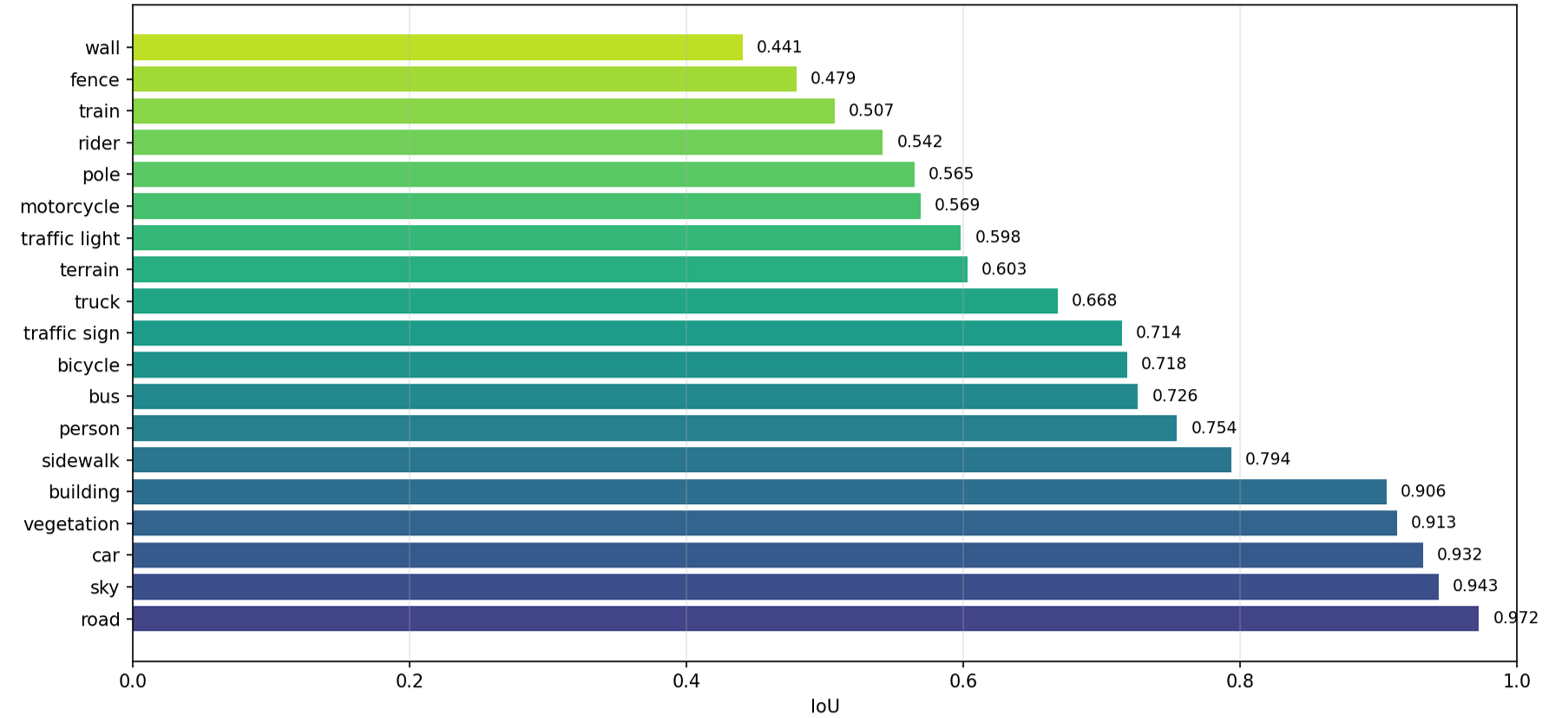
\includegraphics[width=.8\textwidth]{Picture4.png}
  \caption{Per-class IoU after CRF refinement at epoch~22 across all 19 Cityscapes categories.}
  \label{fig:perclass}
\end{figure*}

\begin{figure*}[!b]
  \centering
  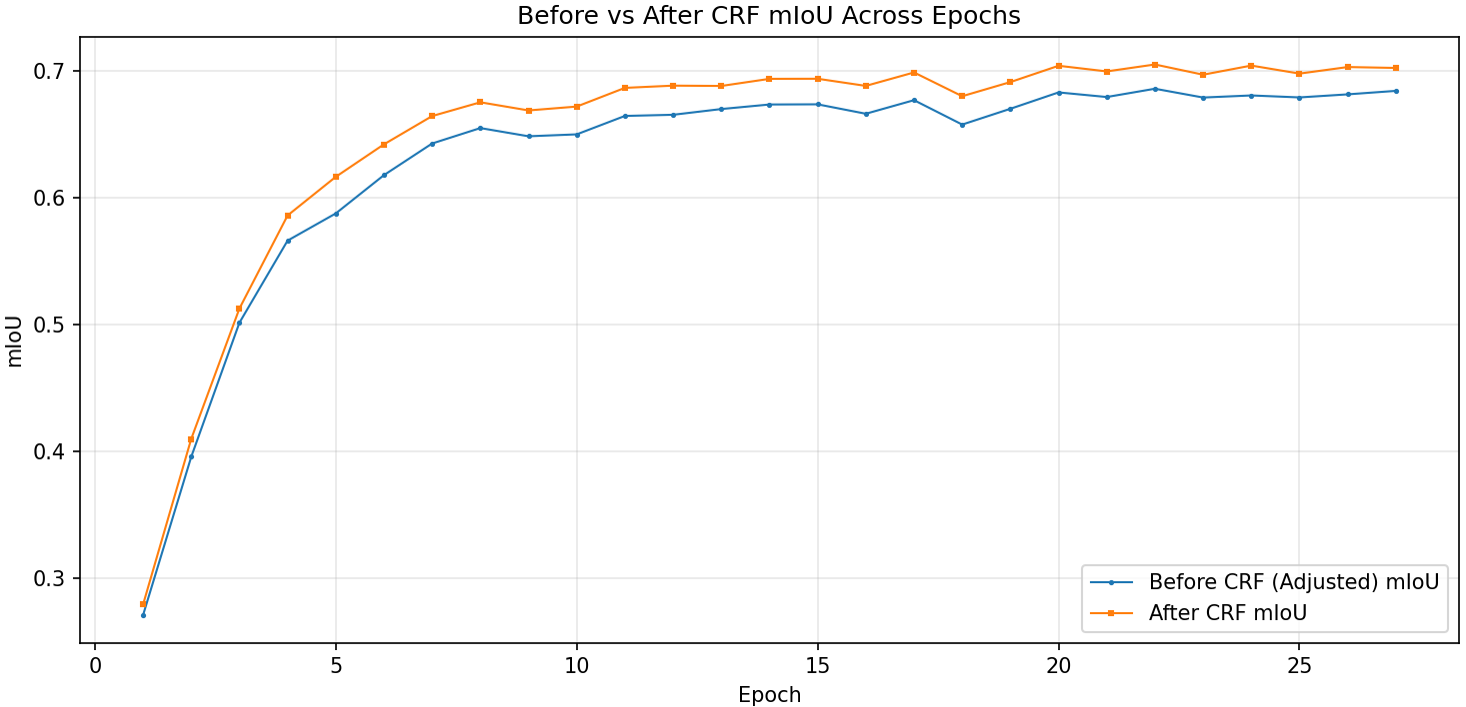
\includegraphics[width=.8\textwidth]{Picture5.png}
  \caption{Validation mIoU before and after CRF refinement across training epochs.}
  \label{fig:training}
\end{figure*}

\subsection{Training Dynamics}\label{subsec:dynamics}

Validation mIoU curves over training epochs before and after CRF refinement are shown in Figure~\ref{fig:training}
below. We observe three distinct phases in the learning dynamics. In the rapid ascent phase (epochs 1-7),
both curves rise sharply from 0.27 to 0.65--0.67 mIoU. This relates to the 1st cosine-annealed warmup
period, where the model learns dominant class boundaries and coarse scene layout quickly. The two curves
are quite similar in this phase, which means that the CRF modules are still optimizing their parameters
and contributing very little at this initial phase. Epochs 7 to around 15, the model begins to consolidate,
and improvements slow substantially, causing both curves to plateau around the 0.65 -- 0.69 point. At this
point, we first start to see the gap opening up between the before and after CRF curves, with the after-range mIoU consistently sitting $\sim$1.5--2 points higher. This stems from the superiority as the unary
predictions mature which shows no residual boundary and label noise errors, thus helping the CRF spatial
regularization to correct them by a greater degree. Starting in epoch 15, the model quickly stabilizes with
after-CRF mIoU remaining between 0.695 and 0.705. Both curves do both dip at epoch 18 by an
observable but slight amount, which is more of a reflection of the learning rate schedule inflection than
any overfitting at this stage. Best checkpoint is decayed at epoch 22, after-CRF mIoU peaks (70.52\%)
with mDice (81.62\%) and pixel accuracy (94.9\%). Model converged without overfitting, with early
stopping displayed after epoch 27.
\begin{figure*}[!t]
  \centering
  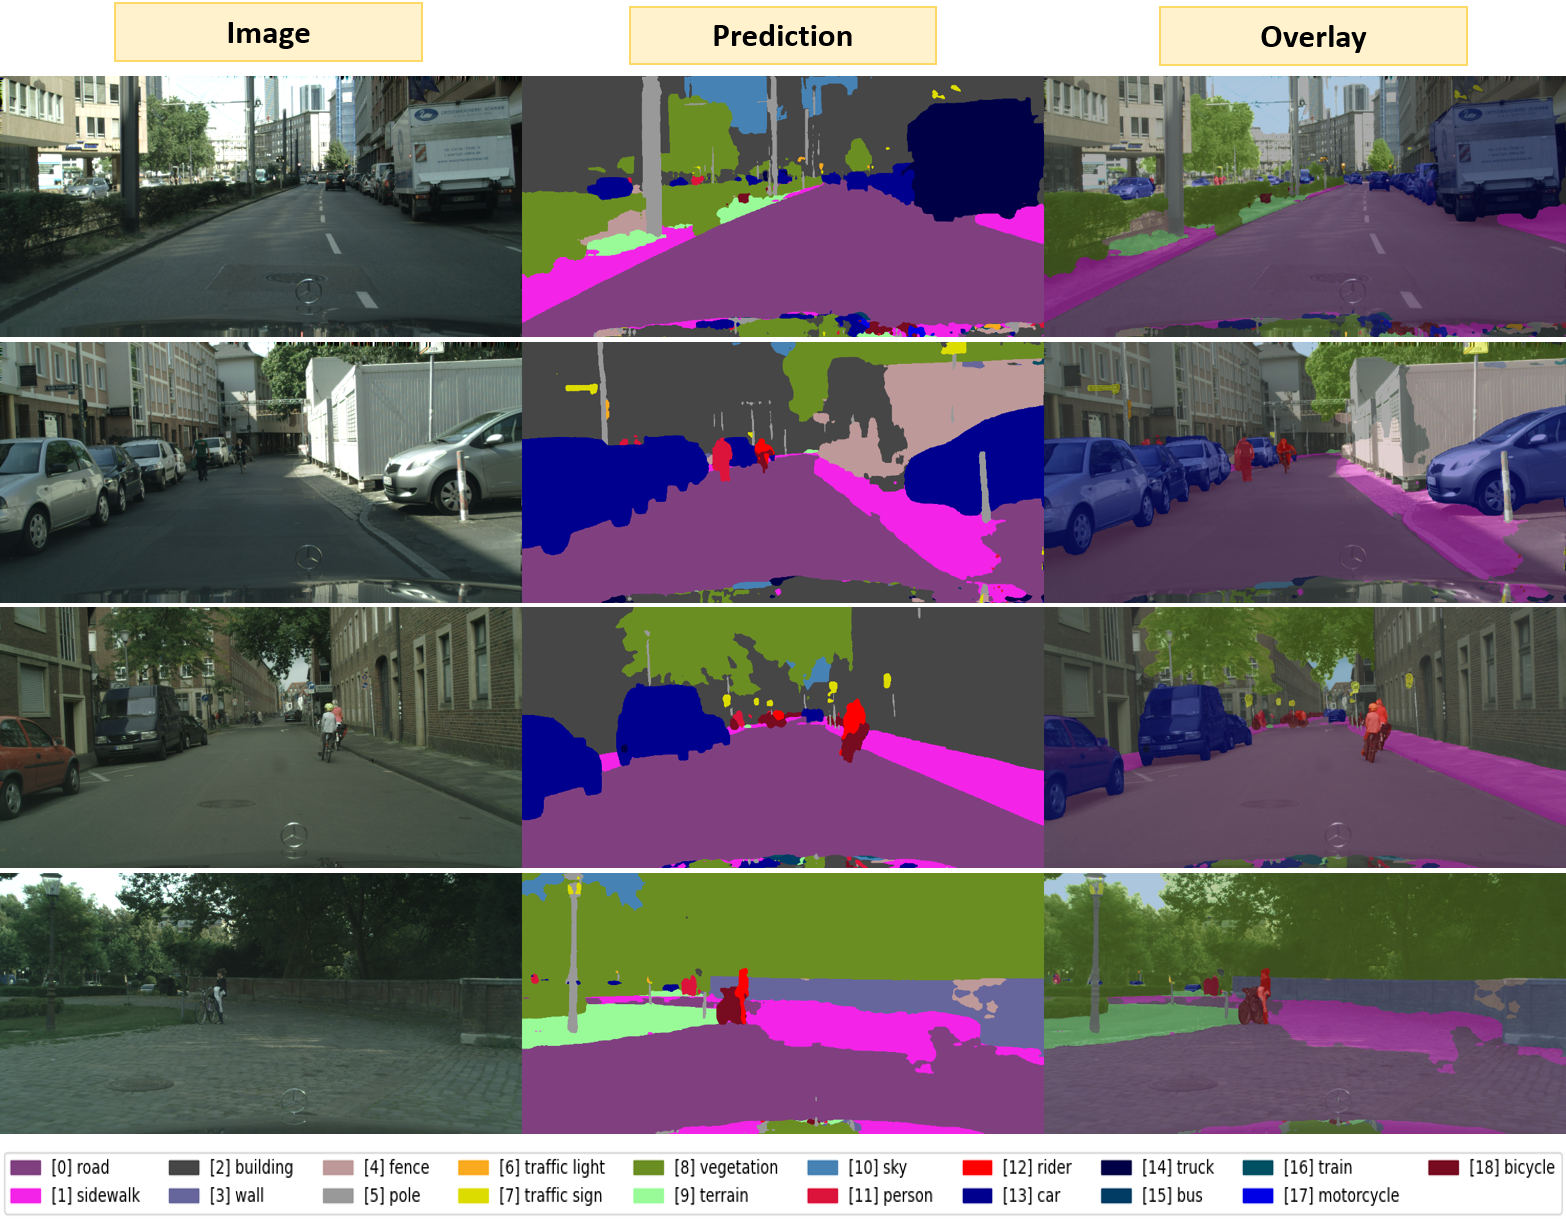
\includegraphics[width=.9\textwidth]{Picture6.png}
  \caption{Qualitative segmentation results showing input image, predicted mask, and overlay for four representative Cityscapes validation scenes.}
  \label{fig:qualitative}
\end{figure*}

\subsection{Qualitative Results}\label{subsec:qual}







Qualitative segmentation results (input image, predicted, and semi-transparent overlay) for four
representative Cityscapes validation scenes are shown in Figure~\ref{fig:qualitative}. The model is capable of performing
well on this problem in general; across all four scenes, the model performs strongly regarding the two
dominant structural classes. Road surfaces are segmented with almost complete spatial coverage and clean
boundaries, consistent with the 0.972 IoU reported quantitatively. Regions such as building facades,
vegetation, and sky are also clearly defined with clean, consistent region boundaries that obey the
geometry of the object underneath. The overlay visualizations show that these large-region predictions are
tightly aligned with their true extents. In scene 1, a narrow urban street scene with the large truck in the
far-right side of the image; the model gets the road, sidewalk, building facades, and the large truck body
correct, and overlap confirms spatial accuracy. The second example, parked cars along a street lined with
buildings, is a moderately well-segmented car scene. The third example (cyclist on an empty street) is a
rather difficult case as well, the rider plus bicycle is localized at a small scale, as different red and dark-red blobs, which correlates with their moderate IoU score. The fourth scene is the hardest (low-light park-like setting with a pedestrian), containing dense vegetation, highly variable terrain, and a semi-occluded
human. The model accurately detects the major vegetation and road/terrain areas, and detects the person,
but its boundary precision is reduced for low-contrast images. In general, qualitative results are aligned
with quantitative results. The model is capable of good performance at large, clean regions and generates
semantically consistent scene-level predictions. This shows that errors are localized with respect to
boundaries of small or rare objects and that this is to be expected, as the per-class IoU distribution suggests
scenes that are low contrast or heavily occluded.



\subsection{Grad-CAM Analysis}\label{subsec:gradcam}

Grad-CAM activation heatmaps calculated at the decoder are shown in Figure~\ref{fig:gradcam}. The first one depicts a
multi-vehicle highway scene, the second is an open urban intersection, and the third is a dense pedestrian
crossing. Here, each column displays the original image and then the top three ranked class activations in
order of ranking. The heatmaps validation indicates that DualPathCRFNet attends to semantically
meaningful and spatially relevant regions for each class. The first scene shown above is of the truck class,
where most activations are concentrated on the body and cargo bed, and more correctly focus on the rear
structure than the road or sky about it. In scene two, the road class activation covers only the entire drivable
surface in a wide, flat activation band, again ignoring the building fa\c{c}ades and signage above, as it should.
The third scene is particularly interesting as the person class activations show that each of the pedestrians
in the busy crossing produces a separate high-energy response, suggesting that the model has acquired
instance-level attention (discriminatively spatial attention for instance classes) for this class, despite the
fact that it was not trained with instance-level supervision. The activation patterns across the three scenes
respect the object boundaries and do not bleed into the surrounding regions significantly, which is
consistent with the role of the frequency-aware edge branch and CRF to refine spatial localization in the
learned feature space.

\begin{figure*}[!t]
  \centering
  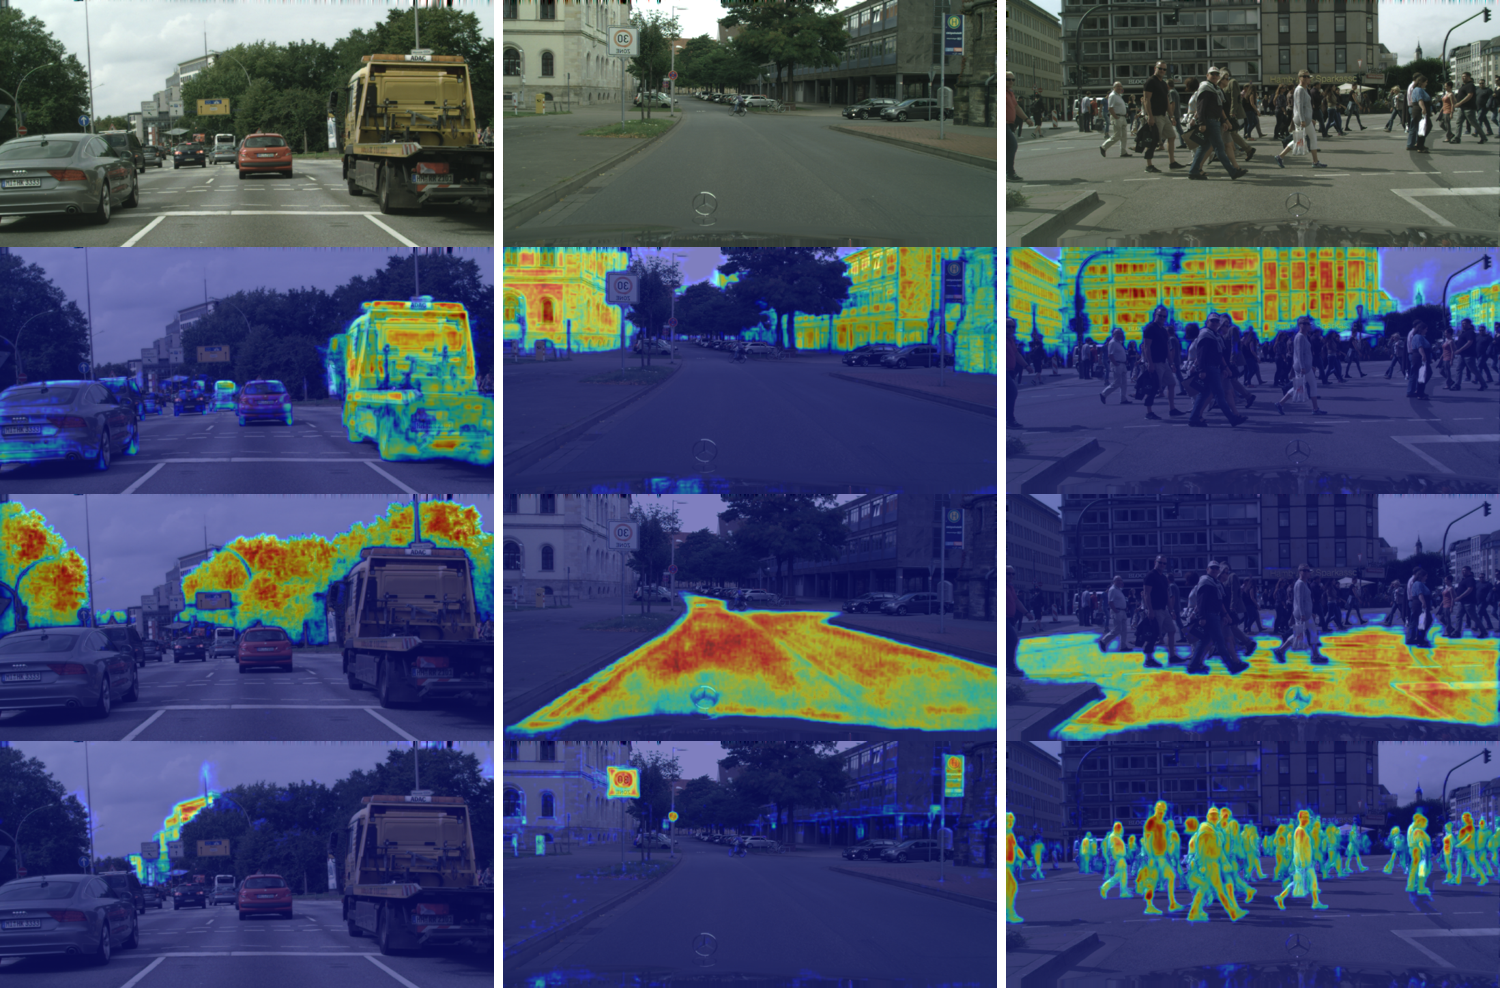
\includegraphics[width=.8\textwidth]{Picture7.png}
  \caption{Grad-CAM class activation heatmaps at the decoder feature layer for
           three urban scenes demonstrating spatially discriminative model attention.}
  \label{fig:gradcam}
\end{figure*}

\begin{figure*}[!t]
  \centering
  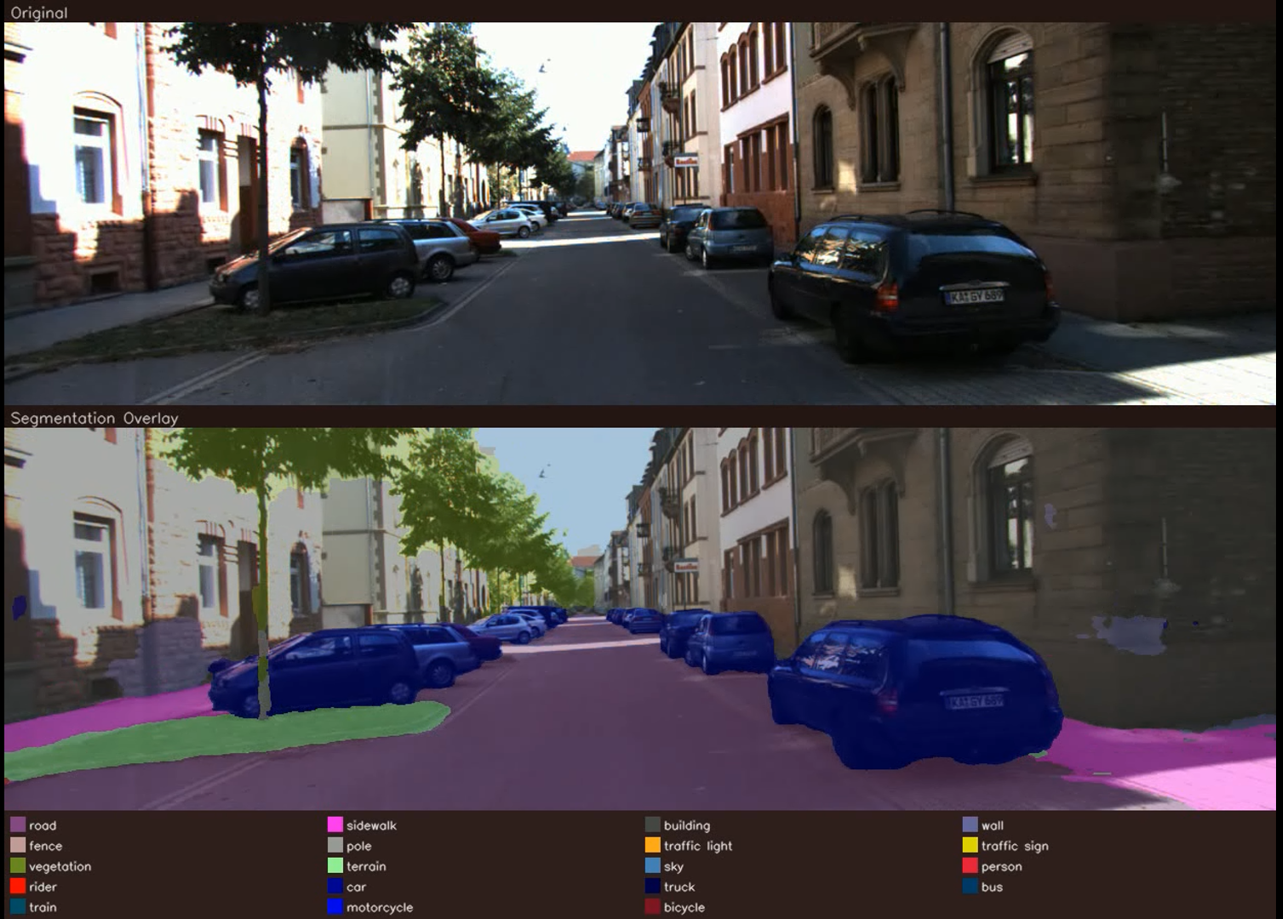
\includegraphics[width=.9\textwidth]{Picture8.png}
  \caption{Qualitative segmentation results of DualPathCRFNet on KITTI driving footage.}
  \label{fig:kitti}
\end{figure*}




\subsection{Cross-Domain Evaluation on KITTI}\label{subsec:kitti}

In order to evaluate the generalizability of DualPathCRFNet beyond the Cityscapes benchmark, we use
real footage of driving to provide an external validation on the KITTI dataset~\cite{geiger2012kitti}. This is a zero-shot domain
transfer evaluation because KITTI was not included in the training or fine-tuning datasets, unlike
Cityscapes. It loaded the model from the best checkpoint and applied it frame by frame to the video
sequences. Predictions were colored using the Cityscapes class palette and overlaid on the original frames.
Even though the camera setup, scene geometry, and image statistics were different from the data used to
train the model, it produced semantically meaningful (large structures like roads, vegetation, buildings,
and vehicles looked visually similar across different domains) segmentation on all scenes. We show an
example of inference video qualitatively on top of KITTI footage below.\\
\url{https://drive.google.com/drive/folders/1xSBRb6HHgNF29E_rqHqHfapDdWPtAJF8?usp=sharing}


 
\section{Discussion}\label{sec:discuss}

Despite the competitive performance of DualPathCRFNet on the Cityscapes benchmark, several
limitations remain that motivate future investigation. The most prominent limitation is the persistent
underperformance on rare and structurally thin classes. Wall (0.441), fence (0.479), train (0.507), and pole
(0.565) remain challenging, primarily due to class imbalance and the fundamental difficulty of segmenting
thin structures at pixel level. The current loss formulation applies a fixed auxiliary weight across all classes
without any class-frequency rebalancing. Incorporating class-balanced or online hard example mining
strategies into the loss function could provide more targeted supervision for underrepresented categories.
The CRF-as-RNN implementation approximates dense bilateral filtering with fixed-size convolutional
kernels ($K=5$), which limits the effective range of pairwise interactions. Long-range spatial dependencies, critical for resolving ambiguities across large homogeneous regions or between spatially distant but
semantically related pixels, are not captured within this approximation. Replacing or augmenting the
convolutional message-passing with deformable convolutions or learned sparse attention could extend the
effective receptive field of the CRF modules without prohibitive computational cost. The current backbone
is a ResNet-50 with partially frozen layers. Upgrading to a more powerful backbone such as a Swin
Transformer or ConvNeXt, with a carefully tuned unfreezing schedule, would likely yield meaningful
gains in semantic feature quality, particularly for the ambiguous mid-range classes where discriminative
representation matters most. Inference time of 103.2 ms per image at 512$\times$1024 resolution currently
precludes real-time deployment. The three cascaded CRF modules are the primary bottleneck. Future work
could explore distilling the multi-scale CRF refinement into a single lightweight module, or applying the
full CRF cascade only during training while using a cheaper approximation at inference. Finally,
evaluating DualPathCRFNet on additional benchmarks such as ADE20K or PASCAL VOC would better
establish the generalizability of the dual-path design beyond urban driving scenarios.

Although DualPathCRFNet performs competitively on the Cityscapes benchmark, there are still a number
of limitations that highlight the need for future work. One major caveat is its difficulties on rare and
structurally thin classes, which simply fail to learn. Segmentation of wall (0.441), fence (0.479), train
(0.507), and pole (0.565) is still difficult, due to the class imbalance and the inherent difficulty of pixel-accurate segmentation of such thin structures. Fixed auxiliary weight across all classes, which does not
perform any class frequency rebalancing at this point of loss formulation. Class-balanced or online hard
example mining strategies in the loss function can be used to query less-well-represented categories more
strongly. The second implementation is CRF-as-RNN, which approximates dense bilateral filtering with
fixed-size ($K = 5$) convolutional kernels, restricting the possible pairwise interactions. This approximation
neglects the long-range spatial dependencies that are essential for resolving ambiguities over large
homogeneous areas, or between spatially separated, but semantically relatable pixels. Using deformable
convolutions or learned sparse attention instead of or in addition to convolutional message-passing would
drastically increase the effective receptive field of the CRF modules without prohibitive computational
overhead. The backbone is the current ResNet-50 with some layers frozen. If upgraded to a more powerful
backbone, like a Swin Transformer or ConvNeXt, with an unfreezing schedule tuned to the new
architecture, that will win some semantic feature signal, at least for those ambiguous mid-range classes
where discriminative representation matters most. Real-time deployment is currently hindered by an
inference time of 103.2 ms per image at 512$\times$1024 resolution. Future work stands to investigate
distillation of the multi-scale CRF refinement into a single lightweight module, or to run the entire CRF
cascade only at training and a faster approximation at inference. Lastly, while tests on the Cityscapes
validate the dual-path design method for urban driving, it will also be important to evaluate
DualPathCRFNet on additional benchmarks such as ADE20K or PASCAL VOC to determine the
generalizability of this dual-path design beyond urban driving.

 
\section{Conclusion}\label{sec:conclusion}

This paper has introduced DualPathCRFNet, a unified end-to-end semantic segmentation framework that
is designed to overcome three major limitations of current approaches: boundary insensitivity, spatially
inconsistent pixel-wise predictions, and ineffective multi-path feature fusion. The architecture specifically
decouples low-frequency semantic content from high-frequency boundary structure, training with a
ResNet-50 semantic backbone and a dedicated frequency-aware edge branch, each path specializing
independently. A scale-adaptive fusion strategy (LightFusion at fine spatial scales and bidirectional
CrossAttnFusion at coarse scales) guarantees that the two streams cooperate and do not compete. The
spatial consistency through the multi-scale CRF-as-RNN decoder is progressively enforced at three
resolutions, from global label coherence at 1/4 resolution to precise boundary alignment at full resolution.
On the Cityscapes validation set, DualPathCRFNet obtains 70.52\% mIoU and 81.62\% mDice with pixel
acc 94.9\% (post-CRF refinement) against the model size of 34.32M parameters. The cross-training
convergence gap between pre- and post-CRF metrics across all training epochs supports the assertion that
the learnable mean-field inference provides non-trivial spatial regularization on top of the FPN decoder.
Qualitative results and Grad-CAM visualizations confirm that the model predicts spatially coherent,
semantically aligned outputs with localized class-specific activations. Although we still make some
assumption that limits the ability to handle rare and thin structured classes, and cannot be deployed in real-time, our method would pave the way for future probabilistically-correct, boundary-aware semantic
segmentation methods.

\section*{AI Use Disclaimer}
In preparing this submission, AI-assisted tools, including Grammarly and ChatGPT were used
primarily to refine the clarity, grammar, and overall structure of the English writing, as well
as to support high-level brainstorming. All methodological decisions, interpretations, and final
content reflect the author's independent understanding of the course materials and the problem
context.

\section*{Dataset and Code Availability}
The augmented Cityscapes dataset used in this work is publicly available at:
\url{https://www.kaggle.com/datasets/jawadulkarim117/cityscapes/data}

The full project code and implementation are available at:
\url{https://github.com/md-jawad-117/CSE756_Project_DualPathCRFNet}

 
\bibliographystyle{IEEEtran}

\begin{thebibliography}{20}

\bibitem{aarthi2017scene}
S.~Aarthi and S.~Chitrakala,
``Scene understanding --- a survey,''
in \emph{Proc. Int. Conf. Computer, Communication and Signal Processing (ICCCSP)},
Jan.~2017, pp.~1--4.
doi:~10.1109/icccsp.2017.7944094.

\bibitem{hurtado2022semantic}
J.~V. Hurtado and A.~Valada,
``Semantic scene segmentation for robotics,''
in \emph{Elsevier eBooks}, 2022, pp.~279--311.
doi:~10.1016/b978-0-32-385787-1.00017-8.

\bibitem{scabini2025survey}
L.~Scabini \emph{et~al.},
``A comparative survey of vision transformers for feature extraction in texture analysis,''
\emph{J. Imaging}, vol.~11, no.~9, p.~304, Sep.~2025.
doi:~10.3390/jimaging11090304.

\bibitem{sutton2012crf}
C.~Sutton and A.~McCallum,
``An introduction to conditional random fields,''
\emph{Found. Trends Mach. Learn.}, vol.~4, no.~4, pp.~267--373, 2012.
doi:~10.1561/2200000013.

\bibitem{arulananth2024unet}
T.~S. Arulananth \emph{et~al.},
``Semantic segmentation of urban environments: Leveraging U-Net deep learning model
for cityscape image analysis,''
\emph{PLoS ONE}, vol.~19, no.~4, p.~e0300767, Apr.~2024.
doi:~10.1371/journal.pone.0300767.

\bibitem{guo2021segnet}
Q.~Guo and Q.~Dou,
``Semantic image segmentation based on SegNet with CRFs,''
\emph{Procedia Comput. Sci.}, vol.~187, pp.~300--306, Jan.~2021.
doi:~10.1016/j.procs.2021.04.066.

\bibitem{an2023crfnet}
T.~An, J.~Kang, D.~Choi, and K.~Min,
``CRFNet: Context refinement network for semantic segmentation,''
\emph{ETRI J.}, vol.~45, no.~5, pp.~822--835, Oct.~2023.
doi:~10.4218/etrij.2023-0017.

\bibitem{huang2021hyperspectral}
Y.~Huang, Q.~Shen, Y.~Fu, and S.~You,
``Weakly-supervised semantic segmentation in cityscape via hyperspectral image,''
in \emph{Proc. IEEE/CVF ICCVW}, Oct.~2021, pp.~1117--1126.
doi:~10.1109/iccvw54120.2021.00131.

\bibitem{maggiolo2021semisupervised}
L.~Maggiolo, D.~Marcos, G.~Moser, S.~B. Serpico, and D.~Tuia,
``A semisupervised CRF model for CNN-based semantic segmentation with sparse ground truth,''
\emph{IEEE Trans. Geosci. Remote Sens.}, vol.~60, pp.~1--15, Jul.~2021.
doi:~10.1109/tgrs.2021.3095832.

\bibitem{gao2022offroad}
B.~Gao, X.~Zhao, and H.~Zhao,
``An active and contrastive learning framework for fine-grained off-road semantic segmentation,''
\emph{IEEE Trans. Intell. Transp. Syst.}, vol.~24, no.~1, pp.~564--579, Nov.~2022.
doi:~10.1109/tits.2022.3218403.

\bibitem{he2021dars}
R.~He, J.~Yang, and X.~Qi,
``Re-distributing biased pseudo labels for semi-supervised semantic segmentation,''
in \emph{Proc. IEEE/CVF ICCV}, Oct.~2021, pp.~6910--6920.
doi:~10.1109/iccv48922.2021.00685.

\bibitem{sahin2023multispectral}
H.~M. Sahin, T.~Miftahushudur, B.~Grieve, and H.~Yin,
``Segmentation of weeds and crops using multispectral imaging and CRF-enhanced U-Net,''
\emph{Comput. Electron. Agric.}, vol.~211, p.~107956, Jun.~2023.
doi:~10.1016/j.compag.2023.107956.

\bibitem{yu2018bisenet}
C.~Yu \emph{et~al.},
``BiSeNet: Bilateral segmentation network for real-time semantic segmentation,''
in \emph{Proc. ECCV}, 2018, pp.~334--349.
doi:~10.1007/978-3-030-01261-8\_20.

\bibitem{zhang2023sar}
J.~Zhang, Y.~Liu, B.~Wang, and C.~Chen,
``A hierarchical fusion SAR image change-detection method based on HF-CRF model,''
\emph{Remote Sens.}, vol.~15, no.~11, p.~2741, May~2023.
doi:~10.3390/rs15112741.

\bibitem{cordts2016cityscapes}
M.~Cordts \emph{et~al.},
``The Cityscapes dataset for semantic urban scene understanding,''
\emph{arXiv preprint arXiv:1604.01685}, Apr.~2016.
doi:~10.48550/arxiv.1604.01685.

\bibitem{he2016resnet}
K.~He, X.~Zhang, S.~Ren, and J.~Sun,
``Deep residual learning for image recognition,''
\emph{arXiv preprint arXiv:1512.03385}, Dec.~2015.
doi:~10.48550/arxiv.1512.03385.

\bibitem{kirillov2019fpn}
A.~Kirillov, R.~Girshick, K.~He, and P.~Dollár,
``Panoptic feature pyramid networks,''
in \emph{Proc. IEEE/CVF CVPR}, Jun.~2019, pp.~6392--6401.
doi:~10.1109/cvpr.2019.00656.

\bibitem{li2024crossfuse}
H.~Li and X.-J. Wu,
``CrossFuse: A novel cross attention mechanism based infrared and visible image fusion approach,''
\emph{arXiv preprint arXiv:2406.10581}, Jun.~2024.
doi:~10.48550/arxiv.2406.10581.

\bibitem{kiefel2014permutohedral}
M.~Kiefel, V.~Jampani, and P.~V. Gehler,
``Permutohedral lattice CNNs,''
\emph{arXiv preprint arXiv:1412.6618}, Dec.~2014.
doi:~10.48550/arxiv.1412.6618.

\bibitem{geiger2012kitti}
A.~Geiger, P.~Lenz, and R.~Urtasun,
``Are we ready for autonomous driving? The KITTI vision benchmark suite,''
in \emph{Proc. IEEE CVPR}, Jun.~2012, pp.~3354--3361.
doi:~10.1109/cvpr.2012.6248074.

\end{thebibliography}

\end{document}